\documentclass[14pt]{beamer}
\title[]{Data Analysis on Demonetisation Twitter Dataset}
\author [SVECW]{Shri Vishnu Engineering College for Women}
\institute[]{Team - 5}
\date{25 Jan 2017}
\usetheme{Madrid}

\usebackgroundtemplate{\includegraphics[width=\paperwidth]}
%\graphicspath{{/home/tsuser/Desktop/Latex_Slides/Images/}}
\graphicspath{{Images/}}
%\graphicspath{{Images/} {ScreenShots/}}
\begin{document}

\begin{frame}
  \titlepage
\end{frame}

\begin{frame}{Team Members}
   \item Naraharisetty Swetha                         - CSE
   \item Chinka Pushpa                       -         CSE
   \item Vangala Revathi                     -         EEE
\end{frame}

\begin{frame}{Contents}
  \begin{itemize}
  \item Data Science
  \item Demonetisation on Twitter
  \item Data Set
  \item Findings
  \item Tools Used
  \item What we have learnt
  \end{itemize}
\end{frame}

\begin{frame}{Data Science}
  \begin{itemize}
    \item It involves
    \pause
  \item Data Cleansing 
    \pause
  \item Data Preparation 
    \pause
  \item Data Analysis
  \end{itemize}
\end{frame}

\begin{frame}{Twitter Tweets on Demonetisation }
  \begin{center}
    \includegraphics[scale=1.0]{olnotes.jpg}
  \end{center}
\end{frame}

\begin{frame}{Data Set}
  \begin{itemize}
  \item Text
    \pause
  \item Created 
    \pause
  \item Retweet Count
    \pause
  \item Favourited
    \pause
  \item Source status
  \end{itemize}
\end{frame}
\begin{frame}{Findings }
  \begin{itemize}
      \item Sentimental Analysis
     \item Word Cloud
     \pause
     \item  In which time people are most active in Twitter?
     \pause
     \item Users of which platform are mostly using the Twitter?
     \pause
     \item What are type of tweets that are  mostly retweeted?
  \end{itemize}
\end{frame}

\begin{frame}{Sentimental Analysis}
  \begin{center}
    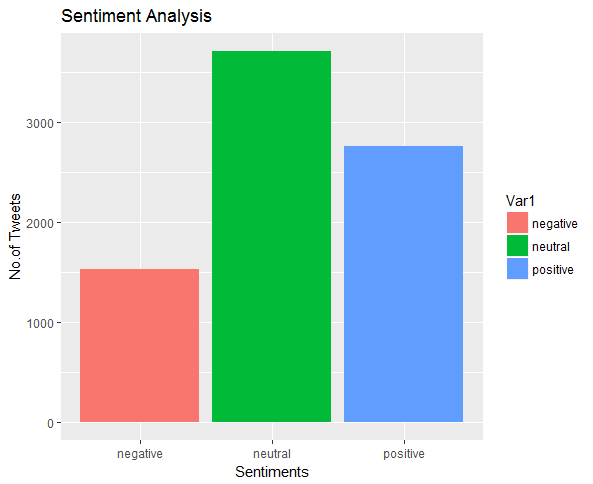
\includegraphics[scale=0.6]{Tweets-Sentiment.png}
  \end{center}
\end{frame}
\begin{frame}{Word Cloud}
  \begin{center}
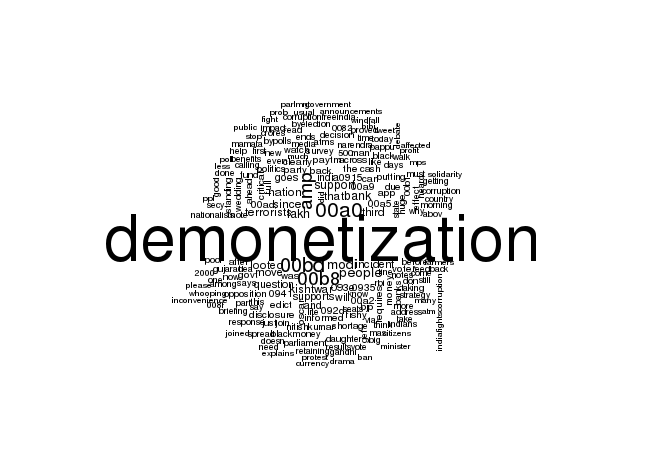
\includegraphics[scale=0.7]{wordCloud.png}
  \end{center}
\end{frame}


\begin{frame}{Time Vs No.of Tweets}
  \begin{center}
    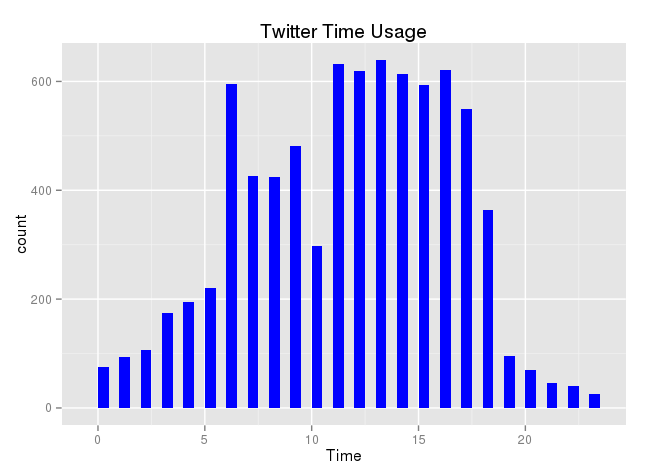
\includegraphics[scale=0.6]{twitter_time.png}
  \end{center}
\end{frame}
\begin{frame}{Platforms Vs No.of Users}
  \begin{center}
\includegraphics[scale=0.65]{final_platfroms.png}
  \end{center}
\end{frame}

\begin{frame}{Reaction of Twitter Users}
  \begin{center}
\includegraphics[scale=0.7]{User_Reaction.png}
  \end{center}
\end{frame}

\begin{frame}{Tools Used}
  \begin{itemize}
     \item R -Studio
     \item Latex Beamer
     \end{itemize}
\end{frame}
\begin{frame}{Packages installed}
     \begin{itemize}
         \item  Sentimentr
         \item  Syuzhet
         \item  Plotrix
         \item  ggplot2
     \end {itemize}
\end{frame}
\begin{frame}{Packages installed}
       \begin{itemize}
          \item Slamx
         \item  Tm
         \item  NLP
         \item  SnowballC
         \item  Wordcloud
         \end{itemize}
\end{frame}
\begin{frame}{What we have learnt}
       \begin{itemize}
           \item How to understand the Dataset?
           \item How to clean the data?
           \item How to Analyse  and Visualise the data?
       \end{itemize}
\end{frame}
\begin{frame}
      \includegraphics[scale = 1.2]{thankyou.jpg}
\end{frame}

\end{document}